\documentclass[12pt,onecolumn,a4paper,fleqn]{article}
\usepackage{epsfig,graphicx,subfigure,amsthm,amsmath}
\usepackage{fancyhdr}
\usepackage{setspace}
\usepackage{sidecap}
\usepackage{tikz}
\usepackage{pgfplots}
\usetikzlibrary{decorations.pathreplacing}
\usepackage{relsize}
\usepackage{color}
\usepackage{ifthen}
\usepackage[framed,numbered]{matlab-prettifier}
\usepackage{files/persianheader}     
\usepackage{float}
\usepackage{enumerate}
\usepackage{booktabs}
\usepackage{xepersian}


\settextfont[Path=fonts/,BoldFont={ZarBd.ttf},BoldFeatures={Scale=0.9}]{BZar.ttf}
\setdigitfont[Path=fonts/,BoldFont={ZarBd.ttf},BoldFeatures={Scale=0.9}]{BZar.ttf}

\pagestyle{fancy}
\fancyhf{}
\rhead{\textbf{علوم اعصاب یادگیری}}
\chead{\textbf{پروژه‌ی پایانی درس}}
\lhead{\textbf{\nouppercase{\rightmark}}}
\cfoot{({\thepage})}
\renewcommand{\headrulewidth}{1pt}
\renewcommand{\footrulewidth}{1pt}
\renewcommand{\sectionmark}[1]{\markright{#1}}
\renewcommand{\subsectionmark}[1]{\markright{#1}}
\newcommand{\pf}[1]{$\mathtt{#1}$}
\onehalfspacing
\begin{document}
	\relscale{1}
	\neurotitlepage

\section*{مقدمه}

توضیحات کلی در مورد کدها و پروژه و مقاله.

\pagebreak

\section{آشنایی با مقاله‌ی پژوهش}

\subsection{هدف پژوهش}
هدف این مقاله مدل سازی \lr{receptive field} نورون‌های پیچیده‌ غشر بصری\footnote{\lr{Visual cortex}} می‌باشد. در واقع با اعمال تحریک‌های تصادفی \lr{spatiotemporal} از توزیع 
$p(s)$
و مشاهده‌ی پاسخ نورون‌ها می‌خواهیم راستایی را بدست بیاوریم که در آن $p(s|r)$ تفاوت معناداری با توزیع اولیه‌ی تحریک‌ها داشته باشد.

تفاوت این مقاله با پژوهش‌های قبل خود آن است که به دلیل رفتار غیر-خطی نورون‌های پیچیده‌ی موجود در \lr{Visual cortex}  نمی‌توانیم از آنالیز‌های خطی 
\lr{spike-triggered average}
که پیش از این کارگشا بودند استفاده کنیم. این مقاله روش 
\lr{spike-triggered correlation analyses}
 را پیشنهاد می‌دهد که بر پایه‌ی \lr{Wiener Kernel} طراحی شده است.

نهایتا با این پژوهش با بررسی‌هایی که انجام می‌دهد ادعا می‌کند که می توان  با این روش پایه‌ای برای تحریک‌ها ارائه داد که تعداد کمی از آن‌ها مشخص کننده‌ی ویژگی‌های مرتبط و تعداد زیادی مربوط به ویژگی‌های پوچ می‌باشند.
\subsection{نورون‌های‌ «پیچیده»}
این مفهوم اولین بار در مقاله‌ی نوبلیست \lr{Hubel and Wiesel} مطرح شده است. نورون‌های ساده نورون‌هایی هستند که رابطه‌ی تحریک-پاسخ آنها نسبت به زمان خطی می‌باشد. این موضوع باعث به وجود آمدن مناطق \lr{ON-OFF} در \lr{Receptive Field} نورون مورد نظر می‌شود. به عکس دست نوشته‌ی موجود در مقاله‌ی مذکور برای جزئیات بیشتر توجه کنید.

\begin{figure}[h]
	\centering
	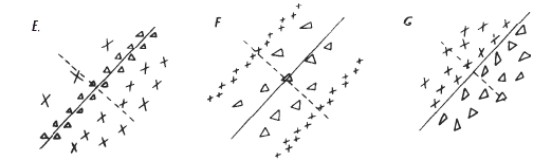
\includegraphics[width=0.8\linewidth]{photos/simple_cells.png}
  \caption[]{مناطق \lr{ON-OFF} حوزه‌ی دریافتی نورون‌های ساده\footnotemark}
\end{figure}
\footnotetext{\lr{EVOLUTION OF IDEAS ON THE PRIMARY
		VISUAL CORTEX, 1955-1978. BY DAVID H. HUBEL}}

همچنین در بخش 
\lr{Material and Methods}
آمده است که اگر نسبت هارمونیک اول به مقدار \lr{DC} حوزه‌ی دریافتی بزرگتر از یک باشد نورون را ساده می‌نامیم. روشن است که نورون‌هایی که از تعاریف بالا پیروی نکنند ساده نبوده و پیچیده‌اند.

\subsection{\lr{STC analysis}}
می‌دانیم که اگر یک ویژگی در تحریک باعث تغییر احتمال اسپایک زدن شود، می‌دانیم که اگه تحریک‌ها را به فضای آن \lr{spike-triggered} منتقل کنیم باید تفاوت قابل توجهی بین مقادیر $p(s|r)$ و $p(s)$ باشد.\footnote{$p(\text{stimulus\ |\ response})$} 

روش‌های مبتنی بر \lr{correlation} با هدف بررسی تغییر این توزیع احتمالات با توجه به تغییرات گشتاور مرتبه‌ی دوم آنها(واریانس) طراحی می‌شوند.

در این بین روش \lr{PCA} به این خاطر که پایه‌ای در اختیار ما قرار می‌دهد که راستا‌های بیشترین تا کمترین واریانس می‌باشند، بسیار مناسب کار ما خواهد بود و می‌تواند ویژگی‌هایی را که در آن واریانس تحریک‌ها بسیار بالا می‌باشد را در اختیار ما بگذارد.

روش \lr{spike-triggered analysis} مبتنی بر موارد فوق مراحل زیر را انجام می‌دهد:
\begin{enumerate}
	\item ابتدا با فرض اینکه حافظه‌ی نورون‌ها بیشتر از ۱۶ فریم یا ۲۶۸ میلی‌ثانیه نخواهد بود؛ پترن‌های تحریک را متشکل از ۱۶ نوار رنگی در ۱۶ فریم و در فضای ۲۵۶ بعدی تعریف می‌کنیم.	
	\item ماتریس \lr{spike-triggered correlation} 
	را به صورت زیر تعریف می‌کنیم:
	$$ C = \frac1N \sum_{i = 1}^{N} S(i)^TS(i) $$
	که در آن $S(i)$ بردار ۲۵۶ بعدی در $i$امین باریست که نورون در طول آزمایش اسپایک زده است و $N$ تعداد کل اسپایک‌ها در طول آزمایش است.
	\item بردارویژه‌ها و مقدارویژه‌های این ماتریس محاسبه شده و با توجه به اندازه‌ی مقدار‌ویژ‌ه‌ها رتبه‌بندی می‌شوند.‌	
\end{enumerate}

با توجه به \lr{PCA} می‌دانیم که حاصل راستا‌هایی خواهد بود که در آن واریانس تحریک‌هایی که موجب اسپایک می‌شوند از زیاد به کم مرتب شده اند.
	
\subsection{اعتبارسنجی نتایج}
برای اعتبارسنجی مشاهدات روش \lr{spike-triggered correlation} روشی که مقاله‌ استفاده می‌کند این است که دنباله‌ای از اسپایک‌های تصادفی با تعداد اسپایک‌های مساوی با $N$ تولید می‌کند و ماتریس \lr{correlation} تحریک‌هایی که موجب این اسپایک‌های فرضی تصادفی شدند را ایجاد می‌کنیم. هدف این است که \lr{control correlation matrix} را محاسبه کنیم که به این معناست که روشی که در قبل پیش گرفتیم را برای داده‌هایی که می‌دانیم مستقل از اسپایک زدن هستند(تمام داده‌ها)نیز اعمال کنیم. با توجه به حجم بالای داده‌ها $N$ مساوی تعداد اسپایک‌ها را در نظر می‌گیریم و ۵ بار فرایند تولید \lr{control correlation matrix} را انجام می‌دهیم و میانگین مقدارویژه‌ها را محاسبه می‌کنیم.با توجه به متن مقاله حاصل این میانگین‌گیری 
$\pm 5.2 SD$ 
بازه‌ی اطمینان ما با $p< 10^{-4}$ خواهد بود. و بنابراین اگر مقدارویژه‌ای خارج از این بازه‌ی اطمینان باشد؛ آن مقدارویژه و بردارویژه دارای تفاوت آشکار خواهند بود.(در واقع آن بردار ویژه راستاییست که تحریک‌های موجب اسپایک در آن واریانس و در نتیجه‌ توزیع احتمال کاملا متفاوتی با توزیع اولیه دارند)
\subsection{نتایج پژوهش}
همانطور که در بخش‌های قبل اشاره کردیم هدف پیدا کردن \lr{eigenvalue}هایی بود که خارج از بازه‌ی اطمینان باشند که آن‌ها به عنوان ویژگی‌های اصلی موجود در \lr{receptive-field} گزارش شود.نتایج مقاله نشان می‌دهد که برای تعداد زیادی از سلول‌های پیچیده دو بردارویژه پیدا شده‌است که این بردار ویژه‌ها ناحیه‌ی \lr{ON-OFF}  مشخص و مجزا ازهمی دارند و همچنین \lr{correlation} بسیار پایینی دارند.همچنین می‌بینیم که این راستا‌ها به خوبی سبب تحریک نورون‌ها می‌شوند با این حال برای \lr{eigenvalue}هایی که در بازه‌ی اطمینان مذکور قرار دارند تاثیر بسیار کمتری در تحریک نورون‌ها مشاهده شده است.

\pagebreak

\section{آشنایی با دیتاست}

\subsection{بخش اول}
با استفاده از تابع تعبیه شده‌ی
	\pf{fget\_hdr.m}
 یکی از فایل‌های \pf{.sa0} را باز می‌کنیم و به محتویات آن توجه می‌کنیم.
 
	\begin{figure}[h]
		\centering
		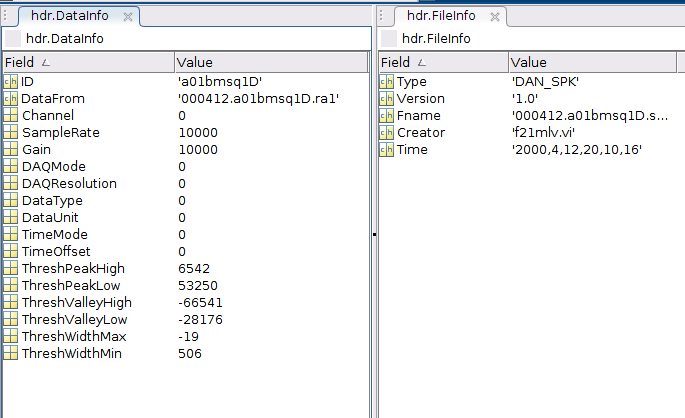
\includegraphics[trim=0.2cm 1cm 0 0.2cm ,clip=true, width=0.8\linewidth]{photos/hdr.png}
		\caption{محتویات فایل \pf{hdr}}
	\end{figure}

می‌توانیم ببینیم که در این فایل اطلاعاتی اطلاعاتی مربوط به خود فایل از جمله‌ زمان ایجاد دیتاست و سازنده‌ی آن و همچنین اطلاعاتی در مورد داده‌ها از جمله نرخ نمونه‌‌گیری وجود دارد.
همچنین در فایل 
\pf{.log} نیز اطلاعاتی مربوط به نورونی که از آن نمونه‌گیری می‌شود وجود دارد.

\begin{table}[h]
	\centering
	\begin{tabular}{|c|c|}
		\hline
		نوع اطلاعات            & برخی از اطلاعات موجود                                \\ \hline
		اطلاعات مربوط به فایل  & زمان ایجاد فایل، سازنده‌ی فایل، ورژن فایل            \\ \hline
		اطلاعات مربوط به تحریک & نوع تحریک، نرخ‌ بروزرسانی مانیتور، نرخ تغییر فریم‌ها \\ \hline
		اطلاعات مربوط به \lr{tuning curve} & زاویه‌‌ی ترجیحی نورون، طول و عرض ترجیحی نورون \\ 
		\hline
				اطلاعات مربوط به نمونه‌‌گیری  & نرخ نمونه‌‌گیری، نوع  کارگذاری الکترود‌ها،  تعداد چنل‌ها         \\ \hline
	\end{tabular}
\end{table}

و اطلاعات دیگری از این دست می‌باشد.

\subsection{بخش دوم}
تابع \pf{Func\_ReadData} را به صورتی که خواسته شده پیاده‌سازی می‌کنیم. ایده‌ی کلی در پیاده‌سازی این تابع این بود که ابتدا با استفاده از تابع \pf{dir} فایل‌های موجود در دایرکتوری نورون مورد نظر را می‌خوانیم و فایل‌های با
\pf{mds1d.sa0}
را پیدا می‌کنیم و اطلاعات آن را با استفاده از 
		\pf{fget\_spk.m}
		می‌خوانیم.
		
		همچنین با توجه به اینکه در بخش بعد به \lr{Spike-count rate} احتیاج پیدا می‌کنیم یکی از خروجی‌های \lr{Optional} را برابر با آن تعریف می‌کنیم، برای محاسبه‌ی این مقدار نیز تنها کافیست توجه کنیم که:
		
		$$ \langle r \rangle = \langle \frac{\#spikes}{time} \rangle_{trials}$$
		
		 نهایتا تابع مورد نظر به صورت زیر خواهد بود:
		


\begin{code}{تابع \pf{Func\_ReadData}}
	\begin{latin}
		\begin{lstlisting}[style=Matlab-editor, tabsize=2]
% Recomend: select Data/ and MatlabFucntions/
% directories and add them to matlab PATH
function [Output, spike_count_rate] = Func_ReadData(NeuronCode)
	Path = [pwd, '/Data', '/Spike_and_Log_Files/', NeuronCode];
	Listing = dir(Path);
	Index_Counter = 0;
	events = {};
	hdrs = {};
	frame_rate = 59.72; %Hz
	frame_number = 32767;
	spike_count = [];
	for i = 1:length(Listing)
		if (contains(Listing(i).name, 'msq1d.sa0', 'IgnoreCase', true) && ...
			~contains(Listing(i).name, 'sa0.sub', 'IgnoreCase', true) && ...
			~contains(Listing(i).name, 'sa0.', 'IgnoreCase', true))
			Index_Counter = Index_Counter + 1;
			[events{Index_Counter}, hdrs{Index_Counter}] = fget_spk(Listing(i).name, 'get');
			spike_count(Index_Counter) = length(events{Index_Counter});
		end
	end
	Output = struct('events', events, 'hdr', hdrs);
	spike_count_rate = mean(spike_count) * frame_rate/frame_number;
end
		\end{lstlisting}
	\end{latin}
\end{code}

\subsection{بخش سوم}
در این بخش ابتدا با استفاده از تابع \pf{dir} در پوشه‌ی مربوط به اطلاعات اسپایک‌ها نام تمام نورون‌ها را استخراج می‌کنیم. سپس با پیمایش بر روی‌ آن‌ها و با استفاده از تابعی که در بخش قبل نوشتیم نرخ اسپایک هر نورون را نگهداری می‌کنیم. نهایتا هیستوگرام نرخ‌ اسپایک‌ها به صورت زیر خواهد بود:

\begin{figure}[h]
	\centering
	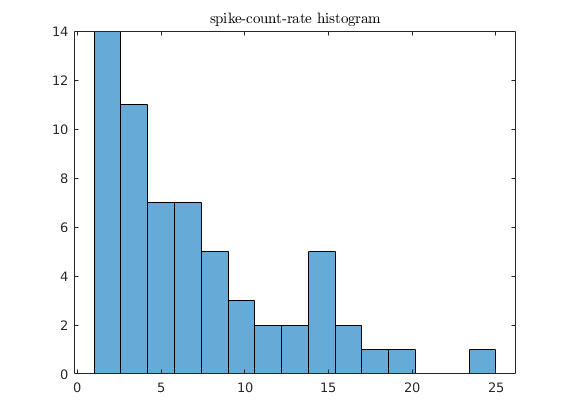
\includegraphics[width=0.6\linewidth]{photos/fr-histogram.png}
	\caption{هیستوگرام نرخ اسپایک‌های نورون‌ها}
	\label{2}
\end{figure}

سپس به سادگی می‌توانیم نورون‌هایی که نرخ اسپایک کمتر از ۲ دارند را با استفاده از قطعه کد زیر از لیست اولیه‌ای که برای کد نورون‌ها تهیه کردیم حذف کنیم.

\begin{code}{حذف نورون‌ها با نرخ اسپایک پایین}
	\begin{latin}
		\begin{lstlisting}[style=Matlab-editor, tabsize=2]
index_counter = 0;
for i = 1:61
	if SCRA(i) < 2
		index_counter = index_counter + 1;
		index(index_counter) = i;
	end
end
fprintf('Exluded Neurons:\n')
disp(neuron_codes(index)')
neuron_codes(index) = [];
		\end{lstlisting}
	\end{latin}
\end{code}


خروجی این قطعه کد شماره‌ی نورون‌های حذف شده را نمایش می‌دهد که به صورت زیر است:
\begin{latin}
	\begin{lstlisting}[basicstyle=\small, frame = single]
Exluded Neurons:
"000413.b03"
"000413.b04"
"000413.b05"
"000418.a01"
"000420.b02"
"000524.c01"
"000907.f07"
	\end{lstlisting}
\end{latin}

\subsection{بخش چهارم}
		در این قسمت تابع \pf{Func\_StimuliExtraction} به گونه‌ای پیاده می‌کنیم که با دریافت دنباله‌ای از زمان اسپایک‌ها تحریک‌هایی با ابعاد 16*16 که سبب این اسپایک‌ها شدند را خروجی بدهد. برای اینکار باید توجه کنیم که با توجه به متن مقاله نرخ تغییر فریم‌های $60Hz$ و به طور دقیق با توجه به فایل‌های لاگ
		 $59.7213Hz$
		 می‌باشد. همچنین از آنجایی که نرخ نمونه برداری $0.1ms$ می‌باشد می‌توان دید که با استفاده از کد زیر می‌تواند اندیس‌هایی از فریم‌ها که در آن‌ها اسپایک رخ‌ داده است را ببینیم.(از آنجایی که تمایل داریم ابعاد ماتریس ۱۶*۱۶ باشد اندیس‌های کمتر از ۱۶ را نادیده در نظر می‌گیریم)

\begin{code}{یافتن اندیس‌های زمان اسپایک و نادیده گرفتن اندیس‌های کمتر ۱۵}
	\begin{latin}
		\begin{lstlisting}[style=Matlab-editor, tabsize=2]
indices = ceil((events * frame_rate) / 10000);
indices = indices(indices>15);
		\end{lstlisting}
	\end{latin}
\end{code}
 
سپس می‌توانیم ماتریس‌های ۱۶*۱۶ که سبب اسپایک شدند را تشکیل دهیم.

برای راحت‌تر شدن کار در مراحل بعد اولا ورودی دوم ذکر شده در صورت سوال یعنی \lr{msq1D} را اختیاری در نظر گرفتیم که مقدار دیفالت آن همان فایلی خواهد بود که در پوشه‌ی \lr{Data} قرار دارد. همچنین در مراحل بعد از آنجایی که می‌خواهیم دنباله‌ای تصادفی از اسپایک‌ها تولید کنیم راحت‌تر خواهد بود که فقط اندیس‌ها را به عنوان ورودی به این تابع بدهیم به این منظور یک ورودی \lr{option} تعریف کردیم که اگر مقدار آن 
\lstinline[style=Matlab-editor, tabsize=2]{'random'}
باشد مقدار \lr{events} در ورودی را به عنوان اندیس‌ها در نظر می‌گیرد و در غیر این صورت همان منطق قبلی را اجرا می‌کند.
		 
\pagebreak

\section{بررسی با روش کلاسیک \lr{STA}}

در کد نهایی که برای این بخش ارائه شده‌ است بر روی تمام ۵۴ نورونی که در بخش قبل حذف نشده‌اند عملیات‌ها صورت می‌گیرد. و حاصل تنها ذخیره می‌شود و تصاویر نمودار‌ها \lr{export} می‌شوند.(بگم دست نزنه یا نگم؟) 

\subsection{بخش اول}
برای محاسبه‌ی این بخش تابع \pf{Func\_FindSTA} پیاده سازی شده است که نحوه‌ی عملکرد آن به صورت زیر است.

\begin{code}{تابع محاسبه‌ی \lr{STA}}
	\begin{latin}
		\begin{lstlisting}[style=Matlab-editor, tabsize=2]
function [sta, spike_trigerred] = Func_FindSTA(neuron)
	outs = neuron.outs;
	spike_trigerred = [];
	for i = 1:length(outs)
		spike_trigerred_trial = Func_StimuliExtraction(outs(i).events);
		spike_trigerred = cat(3, spike_trigerred, spike_trigerred_trial);
	end
	N = length(spike_trigerred);
	sta = (sum(spike_trigerred, 3)/ N);
end		\end{lstlisting}
	\end{latin}
\end{code}

که می‌توان دید بنابر تعریف \lr{STA} پیاده‌سازی شده است. این تابع تمام مقادیر 
\lstinline[style=Matlab-editor, tabsize=2]{spike_trigerred}
را نیز خروجی می‌دهد چرا که در مراحل بعد به آن نیاز خواهیم داشت. برای همان مثالی که در صورت پروژه آمده است خروجی زیر را می‌گیریم:
\begin{figure}[h]
	\centering
	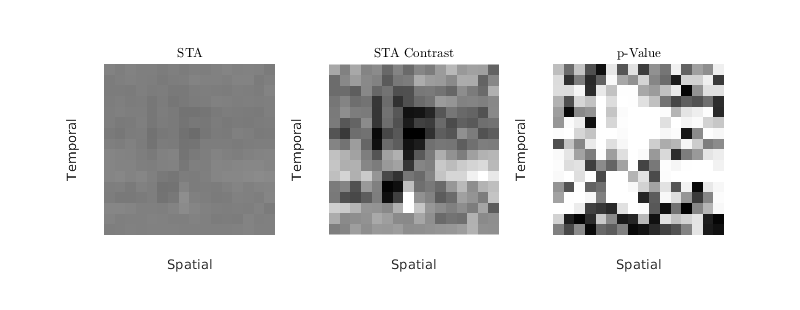
\includegraphics[width=0.5\linewidth]{photos/sta.png}
	\caption{خروجی برای نورون \lr{000601.c05}}
\end{figure}

\subsection{بخش دوم}
خروجی این بخش در بخش اول نمایش داده‌ شد با این حال ذکر می‌کنیم که برای محاسبه‌ی \lr{p-value} به دست آمده از \lr{t-test} از تابع آماده  \pf{ttest}
در متلب استفاده کردیم.
\begin{code}{محاسبه‌ی \lr{t-test}}
	\begin{latin}
		\begin{lstlisting}[style=Matlab-editor, tabsize=2]
[~, p] = ttest(permute(spike_trigerred,[3 1 2]));
	\end{lstlisting}
	\end{latin}
\end{code}

\subsection{بخش سوم}
برای محاسبه‌ی \lr{correlation} از آنجایی که یکی از ماتریس‌هایی که در اختیار ماست ۳بعدی است محاسبه‌ی \lr{correlation} را به صورت دستی انجام دادیم و تابع 
\pf{Func\_Correlation}
را پیاده‌سازی کردیم، که اساس کار آن ضرب درایه به درایه موجود در متلب می‌باشد. همچنین برای تولید دنباله‌ی تصادفی از اسپایک‌ها یا همان ماتریس کنترل به صورت زیر عمل کردیم و در اینجا اضافه کردن پارامتر ورودی اضافه به تابع کارمان را ساده‌تر می‌کند. و تنها کافیست دنباله‌ای تصادفی از شماره‌ی فریم‌ها ایجاد کنیم.
\begin{code}{ایجاد دنباله‌ی تصادفی از تحریک‌ها}
	\begin{latin}
		\begin{lstlisting}[style=Matlab-editor, tabsize=2]
spike_sample = randi([16 32767], 1, N);
stim_control = Func_StimuliExtraction(spike_sample, 'random');
		\end{lstlisting}
	\end{latin}
\end{code}
خروجی هریک از ماتریس‌های کنترل و \lr{spike-triggered} در فضای جدید برای این نورون به صورت زیر است.
\begin{figure}[h]
	\centering
	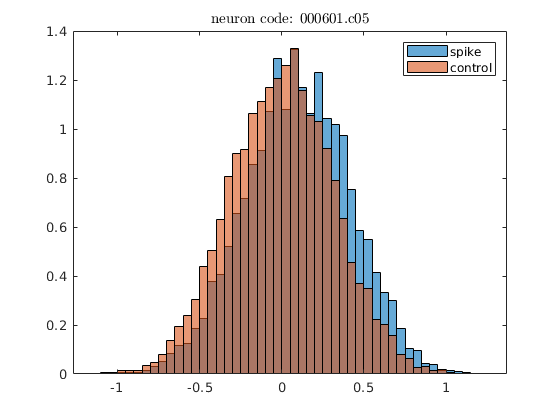
\includegraphics[width=0.46\linewidth]{photos/sta-kernel-hist.png}
	\caption{
		هیستوگرام \lr{correlation} ماتریس‌های کنترل و \lr{spike-triggered} با \lr{STA}
	}
\label{1}
\end{figure}

\subsection{بخش چهارم}
برای محاسبه‌ی \lr{p-value} در اینجا نیز از تابع آماده \pf{ttest2} موجود در متلب استفاده می‌کنیم. خروجی آن به صورت زیر است.

\begin{latin}
	\begin{lstlisting}[basicstyle=\small, frame = single]
p-value = 0.000000, null-hypothesis rejected, means are diffrent.
	\end{lstlisting}
\end{latin}
نتیجه‌ی آزمون \lr{t-test} این است که توزیع‌ $p(s|r)$ و $p(s)$ در فضای مربوط به \lr{STA} دارای میانگین‌های متفاوتی می‌باشند. با این حال با توجه به \autoref{1} برایمان روشن است که این دو توزیع علارغم اینکه میانگین‌های متفاوتی دارند اما به دلیل اینکه‌ سطح مشترک زیر نمودار آنها بسیار زیاد است نمی‌توان تفاوت معناداری بین آنها قائل شد.

به عبارت دیگر نتیجه‌ی آزمون می‌گوید که توزیع‌ $p(s|r)$ و $p(s)$ تفاوت میانگین قابل توجهی دارند که این بر خلاف انتظار ما نمی‌باشد چرا که $p(s|r)$ از تصویر بردارهای منجر به اسپایک بر روی \lr{STA} حاصل می‌شود که واضح است که باید میانگین مثبتی داشته باشد و از طرفی روشن است که با انتخاب تحریک‌های رندم و تصویر کردن روی \lr{STA} میانگینی نزدیک به صفر خواهیم داشت.

با این حال همانطور که از شکل مشخص است تفاوت معنادار در \textbf{میانگین} نمی‌تواند تفاوت معنادار در \textbf{توزیع‌ها} را نشان بدهد و همانطور که از متن مقاله به یاد داریم در آنالیزهایی که بر پایه‌ی \lr{correlation} طراحی می‌شوند تغییر در توزیع‌ها را با تغییر در گشتاور درجه‌ی دوم آنها یا همان واریانس می‌سنجیم.

\subsection{بخش پنجم}
به طور کلی میدانیم که خطای تخمین ما از رابطه‌ی زیر محاسبه می‌شود:
$$ P(\text{Error}) = P(\text{Error}|s=1)P(r=1) + P(\text{Error}|r=0)P(r=0) $$

از طرفی می‌دانیم که با توجه به اینکه تحریک‌های اولیه‌ کاملا تصادفی بودند  $P(s=1)$ همان نرخ اسپایک زدن هر نورون در همین آزمایش می‌باشد. ما قبلا نرخ \lr{spike-count rate} را محاسبه کرده بودیم و از توضیحات درس به یاد داریم که:
$$ P(r=1) = \dfrac{\langle count \rangle}{\Delta t} $$ 
که در اینجا $\Delta t$ همان نرخ تغییر فریم‌ها می‌باشد. حال با توجه به نوع تخمینمان که تنها به یک پارامتر $\theta$ وابسته می‌باشد مقدار خطا را باز نویسی می‌کنیم:

$$ P(\text{Error}) = P(X > \theta | r = 0)P(r = 0) + P(X < \theta | r = 1)P(r = 1) $$

توزیع $P(X|r=1)$ همان توزیع تصویر \lr{spike-triggered } ها بر روی \lr{STA} می‌باشد که طبق فرض مسئله آن را نرمال در نظر می‌گیریم. از طرف دیگر با توجه به \lr{sparse} بودن نورون‌ها و احتمال پایین اسپایک زدن آنها(برای اکثر نورون‌ها با توجه به \autoref{2} در حدود $10^{-2}$ می‌باشند) می‌توانیم توزیعی که برای تصویر \lr{control} محاسبه کردیم را توزیع $P(X|r=0)$ در نظر بگیریم و بنابراین می‌توانیم $P(\text{Error})$ را محاسبه کنیم و مشتق آن نسبت $\theta$ را برابر با صفر قرار دهیم تا بهترین ترشهولد را محاسبه کنیم.

برای محاسبه این مقادیر در متلب ابتدا یک فیت گاوسی بر روی هیستوگرام‌ها ایجاد می‌کنیم و سپس $\mu$ و $\sigma$ را محاسبه می‌کنیم و آن‌ها را به همراه احتمال اسپایک زدن نورون به تابع نوشته شده‌ی
 \pf{Func\_Accuracy} می‌دهیم که ترشهولد و دقت تخمین ما را بیان می‌کند.

\begin{figure}[h]
	\centering
	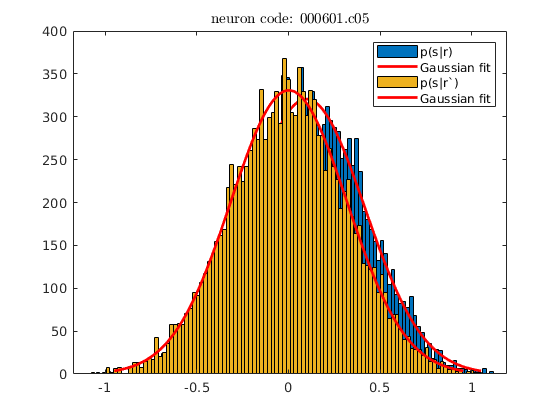
\includegraphics[width=0.6\linewidth]{photos/sta-fit-gaussian.png}
	\caption{
هیستوگرام‌ها به همراه فیت گوسی آن‌ها
	}
	\label{1}
\end{figure}

همچنین توجه می‌کنیم که برای محاسبه‌ی 
\pf{Func\_Accuracy}
از سایت‌های محاسبه کننده استفاده کردیم و خروجی آنها را در تابع متلب قرار دادیم.
 
\pagebreak
		 
		 \subsection{بخش ششم}
		 با اجرای مراحل بالا برای تمامی ۵۴ نورون باقی مانده به خروجی‌های زیر دست پیدا می‌کنیم لازم است توجه کنیم که داده‌های کنترل به صورت رندم تولید می‌شوند و بنابراین با اجرای این کدها ممکن است نتایج اندکی متفاوت بگیریم هر چند در کلیت پاسخ تاثیری نخواهند داشت.
	
		 \newcounter{int}
		 \setcounter{int}{1}
		 \loop
		 
		 \begin{figure}[ht]
		 	\centering
			\subfigure{\includegraphics[width=0.55\linewidth]{photos/STA/imshows/\theint.png}}
			\hfill
			\subfigure{\includegraphics[width=0.4\linewidth]{photos/STA/histograms/\theint.png}}
		 \end{figure}
		 
		 \addtocounter{int}{1}\ifnum\value{int}<10
		 \repeat
		 
		 
		 \loop
		 
		 \begin{figure}[h]
		 	\centering
		 	\subfigure{\includegraphics[width=0.55\linewidth]{photos/STA/imshows/\theint.png}}
		 	\hfill
		 	\subfigure{\includegraphics[width=0.4\linewidth]{photos/STA/histograms/\theint.png}}
		 \end{figure}
		 
		 
		 \addtocounter{int}{1}\ifnum\value{int}<18
		 \repeat
		 
		 \clearpage
		 
		 \loop
		 
		 
		 \begin{figure}[h]
		 	\centering
		 	\subfigure{\includegraphics[width=0.55\linewidth]{photos/STA/imshows/\theint.png}}
		 	\hfill
		 	\subfigure{\includegraphics[width=0.4\linewidth]{photos/STA/histograms/\theint.png}}
		 \end{figure}	 	     

		 
		 \addtocounter{int}{1}\ifnum\value{int}<55
		 \repeat 
		 
		 
		 \clearpage
		 
		\subsection{بخش هفتم}
	با اینکه میانگین توزیع‌ها با توجه به تست‌های آماری با هم تفاوت دارند از آنجایی که تقریبا تمامی نمودار‌های رسم شده نشان می‌دهند که توزیع تصویر تحریک‌ها بر راستای \lr{STA} برای کلیه تحریک‌ها و تحریک‌هایی که موجب اسپایک شدند تفاوت چشمگیری با هم ندارند و به درستی نمی‌توان ترشهولدی پیدا کرد که با انتخاب آن داده‌ها را با دقت خوبی بتوان دسته‌بندی کرد.از طرف دیگر مولفه‌ی \lr{STA} در بیشتر نورون‌ها الگوی‌ معناداری ندارد و بیشتر شبیه نویز‌ می‌باشد.به عبارتی تا حد خیلی زیادی می‌توان به اعای مقاله مبنی بر پیچیدگی نور‌ون‌هایی که با آنها سروکار داریم استناد کرد.
	
	با این وجود می‌توان دید که برخی از نورون‌های جدولی که در بالا ارائه کردیم نه تنها پترنی با الگوی معنادار دارند بلکه نمودار توزیع آن‌ها به علت تفاوت \textbf{میانگین} که باهم دارند را به خوبی می‌توان تفکیک کرد از بین این‌ها اطلاعات 
		
		 
		 
		 
		
\end{document}